\documentclass[ngerman]{scrartcl} %lädt die Dokumentklasse
                                %Artikel von Koma-Skript, als Option
                                %übergebe ich, dass ich die Trennung
                                %nach neuer deutscher Rechtschreibung
                                %wünsche

\author{Jawoon Kim, Charlie Wiegand}
\usepackage[ngerman]{babel}
\usepackage[utf8]{inputenc}
\usepackage{color}
\usepackage[a4paper,lmargin={4cm},rmargin={2cm},tmargin={2.5cm},bmargin = {2.5cm}]{geometry}
\usepackage{amssymb}
\usepackage{amsthm}
\usepackage{graphicx}
 \begin{document}
 \begin{titlepage}
	\section{}
	\centering
	
\includegraphics[width=0.3\textwidth]{images/arc42-logo.png}\par\vspace{1cm}
	{\scshape\LARGE bib International College\par}
	\vspace{1cm}
	{\rmfamily\scshape Lernaufgabe 2020\par}
	\vspace{1.5cm}
	{\Huge\bfseries bib now\par}
	\vspace{2cm}
	{\Large\itshape Charlie Wiegand\par Jawoon Kim\par}
	\vfill
	betreut von Frau Langeheinecke\par
	\vfill
	{\large \today\par}
\end{titlepage}

 \maketitle
\title{bibnow}
\vspace{2cm}

\section{Über bibnow}
bib-now, das Forum, das exclusive Forum für alle Studierenden und Mitarbeiter.

\vspace{1cm}

Erstellt von Jawoon Kim und Charlie Wiegand(PBT3H19A).

Letzte Revision: September 2020

\vspace{2cm}

\begin{quote}
\textbf{Note}

Diese Version enthält die Dokumentation der Webseite und Erläuterungen. Sie dient
der Einarbeitung in bib-now sowie dem Verständnis der Konzepte. 
\end{quote}

\pagebreak

\hypertarget{_aufgabenstellung}{%
\subsection{Aufgabenstellung}
\label{_aufgabenstellung}}

\textbf{Inhalt.}

Da zur Zeit häufig Mails an die ganze Schule geschickt werden, wenn beispielsweise jemand etwas verloren hat, wollen wir unseren Mitschülern und uns ein Forum bieten, das diesen Austausch erleichtert.

Für dieses Vorhaben haben wir uns folgende Ziele und Richtlinien gesetzt

\begin{itemize}
\item
\textbf{Minimum}
  Es soll eine lauffähige Webseite erstellt werden, auf der man sich mindestens einloggen kann und anschließend Beiträge in Textform hochladen kann. 
\item
\textbf{Optional}
  Es soll die Möglichkeit geben seine Beiträge durch Bilder zu ergänzen und die Posts sollen in Kategorien eingeteilt werden
\item
\textbf{Optional}
Desweiteren soll es die Möglichkeit den Stundenplan und Klausurplänung aus dem offiziellen Intranet zu übernehmen.

\end{itemize}


\textbf{Vorausetzungen}
Um das Minimum zu erreichen benötigen wir einen PC, einen Texteditor, npm, ein AngularFramework und Firebase. Um uns die Zusammenarbeit zu erleichtern haben wir uns entschieden Versionskontrolle über git laufen zu lassen und die Ergebnisse über GitHub auszutauschen. 

\section{Konzepte}
\label{section-konzepte}}

\textbf{Inhaltskonzept}

\vspace{2cm}
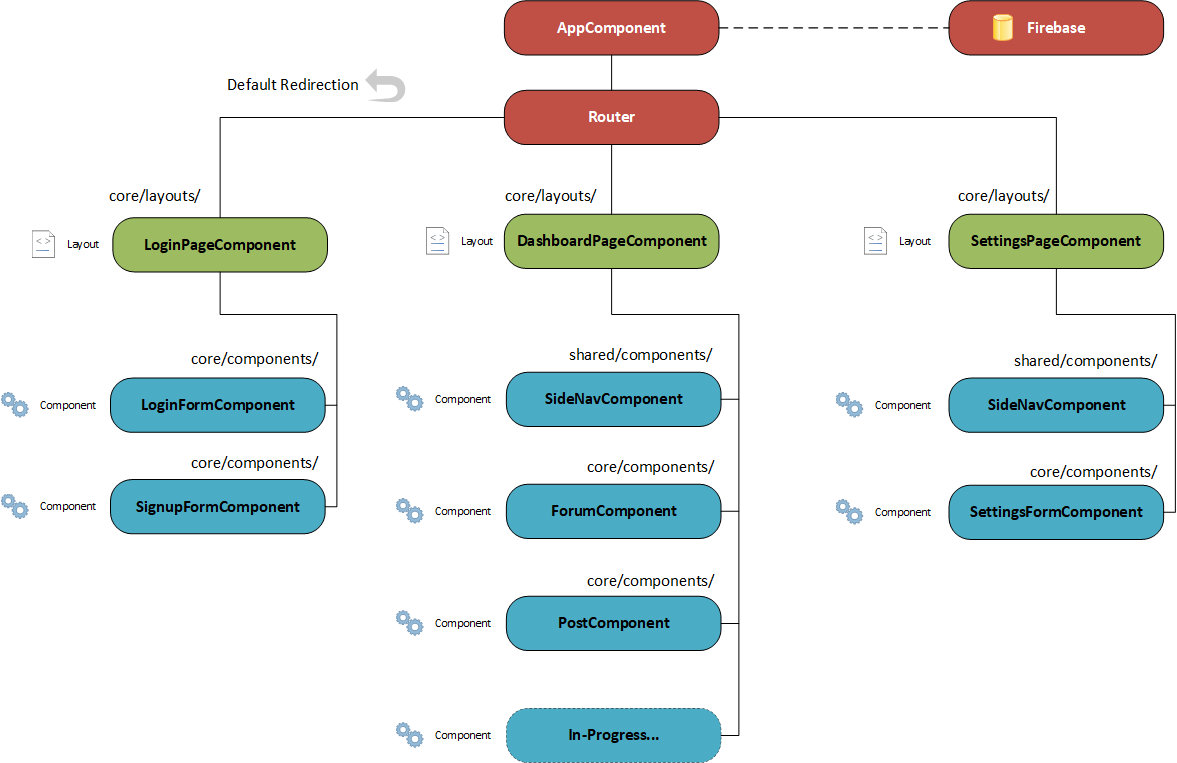
\includegraphics{./Konzepte/bibnow_Sitemap.png}
\vspace{2cm}

%Inhaltskonzept (TODO)
Bei bib-now handelt es sich um ein Schülerforum für das bib international College Paderborn. Die technische Umsetzung basiert auf  einer Single-Page-Webanwendung mit einer RealTime-Datenbank deren einzelnde Komponenten über einen Router verlinkt sind: Die Navigation besteht aus drei Komponenten: LoginPageComponent, DashboardPageComponent und der SettingsPageComponent. Jede dieser Komponenten besitzt ihre eigenen Backend-Komponenten. Die LoginPage greift auf die LoginFormComponent und SignUpFormComponent zurück. Die DashboardPageComponent greift auf  SideNavComponent, ForumComponent, PostComponent zurück. Außerdem könnnen hier später weitere Elemente ergänzt werden. SettingsPageComponent beinhaltet die SideNavComponent und SettingsFormComponent. 


\pagebreak

\textbf{Navigationskonzept}

\vspace{2cm}
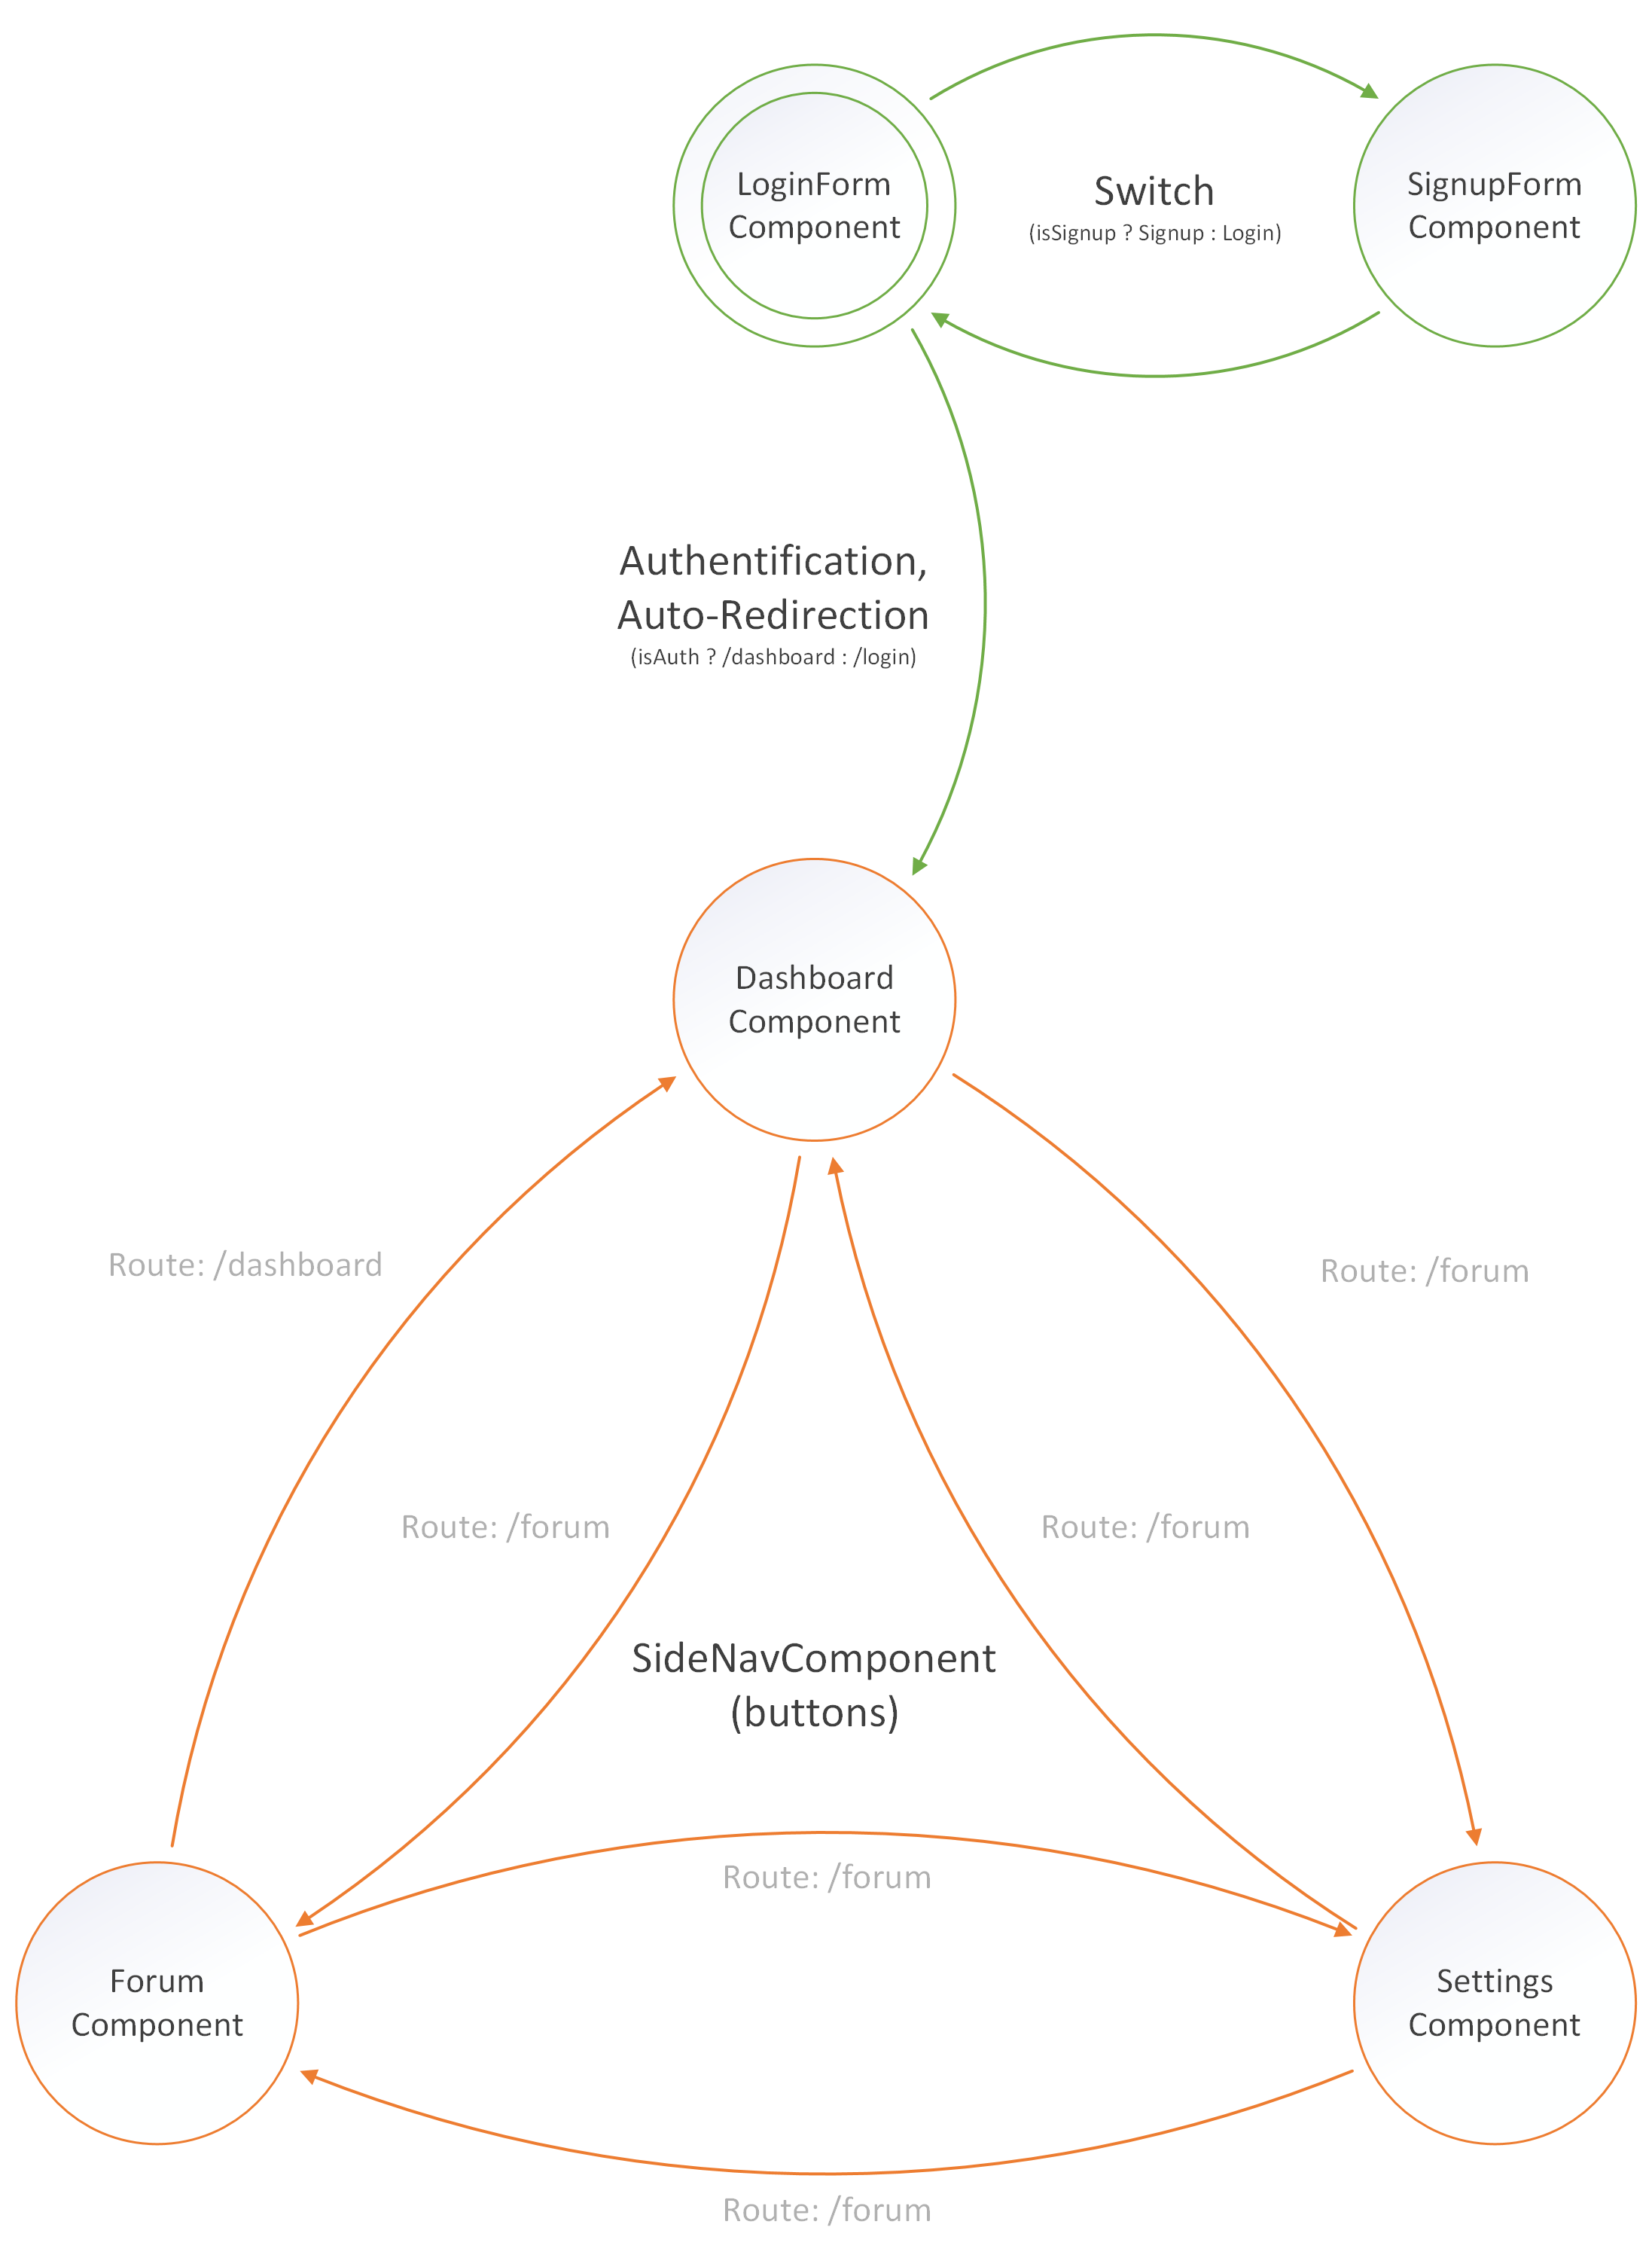
\includegraphics{Konzepte/bibnow_Navigationskonzept.png}
\vspace{2cm}

%Inhaltskonzept (TODO)
Beim Betreten der Seite wird der User zunächst aufgefordert sich einzuloggen. Sollte er sich noch nicht registriert haben hat er die Möglichkeit in das Registrierungsforumlar zu switchen und sich dort zu registrieren. War die Registrierung oder das einloggen erfolgreich, wird der User auf die DashboardPage weitergeleitet. Dort werden ihm Posts angezeigt und er hat die Möglichkeit über ein Formular einen eigenen Post zu verfassen. Außerdem kann er über das Navigationsmenu zu der SettingsPage zu wechseln. Seine aktuelle Position wird durch eine Farbveränderung am jeweiligen punkt in der Navigatonsleiste erkenntlich.


\textbf{Gestaltungskonzept}

Font: Montserrat (https://fonts.google.com/specimen/Montserrat)
Font Weights: 100, 300, 700
\vspace{2cm}
\begin{itemize}
\item
	Für Subtiteln, gedämpfte Texte, etc


\includegraphics{images/Schriftart_100.png}
\item
	Für normale Texte, Standard-schriftart


\includegraphics{images/Schriftart_300.png}
\item
	Für Titeln und Akzent(Betonung)


\includegraphics{images/Schriftart_700.png}
\end{itemize}


Farbenschema

Schemakonzept: Neon + Material

Primärfarbe: #D43D61
Sekundär: #039BE5
Hintergrund: #271D33
Hintergrund Beiträge: #F8F6F6

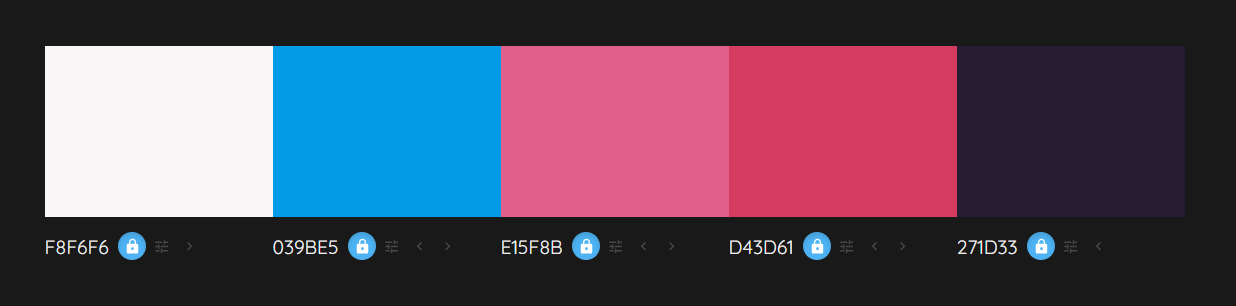
\includegraphics{images/Schema_1.png}
\end{document}
